\hypertarget{test__replace2_8cpp}{}\subsection{test\+\_\+replace2.\+cpp File Reference}
\label{test__replace2_8cpp}\index{test\+\_\+replace2.\+cpp@{test\+\_\+replace2.\+cpp}}


Contains an example to take subject string, replacement string, modifier and pattern from user input and perform regex replace with J\+P\+C\+R\+E2.  


{\ttfamily \#include $<$iostream$>$}\newline
{\ttfamily \#include \char`\"{}jpcre2.\+hpp\char`\"{}}\newline
Include dependency graph for test\+\_\+replace2.\+cpp\+:\nopagebreak
\begin{figure}[H]
\begin{center}
\leavevmode
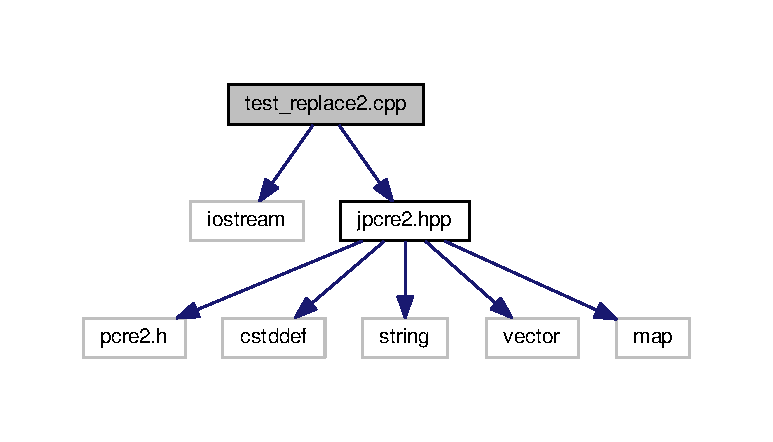
\includegraphics[width=350pt]{test__replace2_8cpp__incl}
\end{center}
\end{figure}


\subsubsection{Detailed Description}
Contains an example to take subject string, replacement string, modifier and pattern from user input and perform regex replace with J\+P\+C\+R\+E2. 


\begin{DoxyCodeInclude}

\textcolor{preprocessor}{#include <iostream>}
\textcolor{preprocessor}{#include "\hyperlink{jpcre2_8hpp}{jpcre2.hpp}"}


\textcolor{preprocessor}{#define getLine(a) std::getline(std::cin,a,'\(\backslash\)n')}


\textcolor{keywordtype}{int} main()\{
    std::string pat,mod,subject,repl,repl\_mod;

    std::cout<<\textcolor{stringliteral}{"\(\backslash\)nEnter pattern: "};
    getLine(pat);

    std::cout<<\textcolor{stringliteral}{"\(\backslash\)nEnter compile modifiers (eijmnsuxADJSU): "};
    getLine(mod);
    \hyperlink{classjpcre2_1_1Regex}{jpcre2::Regex} re;   

    \textcolor{comment}{// Compile the pattern}
    re.\hyperlink{classjpcre2_1_1Regex_aad1d5ef1e87f762f68a587eec4022e69_aad1d5ef1e87f762f68a587eec4022e69}{compile}(pat,mod);
    
    \textcolor{comment}{//check if it was a success}
    \textcolor{keywordflow}{if}(!re)\{std::cerr<<re.\hyperlink{classjpcre2_1_1Regex_a8606fff8b192c94f58ca9e82aa048c61_a8606fff8b192c94f58ca9e82aa048c61}{getErrorMessage}();\} 
    
    \textcolor{comment}{//if(re) is only available for >=C++11, use if(!!re) as an alternative}
    
    \textcolor{comment}{/* // >= C++11}
\textcolor{comment}{    if(re) std::cout<<"\(\backslash\)n Success";}
\textcolor{comment}{    else std::cout<<"\(\backslash\)n Failure";}
\textcolor{comment}{    */}
    
    \textcolor{keywordflow}{if}(!!re) std::cout<<\textcolor{stringliteral}{"\(\backslash\)n Compile Success"};
    \textcolor{keywordflow}{else} std::cout<<\textcolor{stringliteral}{"\(\backslash\)n Compile Failure"};

    \textcolor{comment}{// subject string}
    std::cout<<\textcolor{stringliteral}{"\(\backslash\)nEnter subject string (enter quit to quit): "}<<std::endl;
    getLine(subject);
    \textcolor{keywordflow}{if}(subject==\textcolor{stringliteral}{"quit"})\textcolor{keywordflow}{return} 0;
    
     \textcolor{comment}{//replacement string}
    std::cout<<\textcolor{stringliteral}{"\(\backslash\)nEnter replacement string: "}<<std::endl;
    getLine(repl);

    std::cout<<\textcolor{stringliteral}{"\(\backslash\)nEnter action (replacement) modifiers (eEgx): "};
    getLine(repl\_mod);

    \textcolor{comment}{//perform replace}

    std::cout<<\textcolor{stringliteral}{"\(\backslash\)nreplaced string: "}<<
        re.\hyperlink{classjpcre2_1_1Regex_ae7235a991492fa88f1bd3fb02d59cd0a_ae7235a991492fa88f1bd3fb02d59cd0a}{initReplace}()
          .\hyperlink{classjpcre2_1_1RegexReplace_a46eefdb105827920bebc8436721fa4cb_a46eefdb105827920bebc8436721fa4cb}{setSubject}(subject)
          .\hyperlink{classjpcre2_1_1RegexReplace_af1069f489de9b343493da2dc77b04c73_af1069f489de9b343493da2dc77b04c73}{setReplaceWith}(repl)
          .\hyperlink{classjpcre2_1_1RegexReplace_a06a57430f62058822d48722a2a6425d7_a06a57430f62058822d48722a2a6425d7}{addModifier}(repl\_mod)
          .\hyperlink{classjpcre2_1_1RegexReplace_afd087fa7a9bfedec802d1a3dd7edbdd0_afd087fa7a9bfedec802d1a3dd7edbdd0}{replace}();

    \textcolor{keywordflow}{return} 0;
\}
\end{DoxyCodeInclude}
 \begin{DoxyAuthor}{Author}
\href{https://github.com/neurobin}{\tt Md Jahidul Hamid} 
\end{DoxyAuthor}
